\documentclass[]{article}
\usepackage{amsfonts}
\usepackage{amsmath}
\usepackage{graphicx}
\usepackage{amsthm}
\usepackage{svg}
\usepackage{enumitem}
\usepackage{color}
\usepackage{float}
\usepackage[utf8]{inputenc}

%%%%% Alphabets %%%%% 
\def\cA{\mathcal{A}}\def\cB{\mathcal{B}}\def\cC{\mathcal{C}}\def\cD{\mathcal{D}}\def\cE{\mathcal{E}}\def\cF{\mathcal{F}}\def\cG{\mathcal{G}}\def\cH{\mathcal{H}}\def\cI{\mathcal{I}}\def\cJ{\mathcal{J}}\def\cK{\mathcal{K}}\def\cL{\mathcal{L}}\def\cM{\mathcal{M}}\def\cN{\mathcal{N}}\def\cO{\mathcal{O}}\def\cP{\mathcal{P}}\def\cQ{\mathcal{Q}}\def\cR{\mathcal{R}}\def\cS{\mathcal{S}}\def\cT{\mathcal{T}}\def\cU{\mathcal{U}}\def\cV{\mathcal{V}}\def\cW{\mathcal{W}}\def\cX{\mathcal{X}}\def\cY{\mathcal{Y}}\def\cZ{\mathcal{Z}}

\def\AA{\mathbb{A}} \def\BB{\mathbb{B}} \def\CC{\mathbb{C}} \def\DD{\mathbb{D}} \def\EE{\mathbb{E}} \def\FF{\mathbb{F}} \def\GG{\mathbb{G}} \def\HH{\mathbb{H}} \def\II{\mathbb{I}} \def\JJ{\mathbb{J}} \def\KK{\mathbb{K}} \def\LL{\mathbb{L}} \def\MM{\mathbb{M}} \def\NN{\mathbb{N}} \def\OO{\mathbb{O}} \def\PP{\mathbb{P}} \def\QQ{\mathbb{Q}} \def\RR{\mathbb{R}} \def\SS{\mathbb{S}} \def\TT{\mathbb{T}} \def\UU{\mathbb{U}} \def\VV{\mathbb{V}} \def\WW{\mathbb{W}} \def\XX{\mathbb{X}} \def\YY{\mathbb{Y}} \def\ZZ{\mathbb{Z}}  

\def\fa{\mathfrak{a}} \def\fb{\mathfrak{b}} \def\fc{\mathfrak{c}} \def\fd{\mathfrak{d}} \def\fe{\mathfrak{e}} \def\ff{\mathfrak{f}} \def\fg{\mathfrak{g}} \def\fh{\mathfrak{h}} \def\fj{\mathfrak{j}} \def\fk{\mathfrak{k}} \def\fl{\mathfrak{l}} \def\fm{\mathfrak{m}} \def\fn{\mathfrak{n}} \def\fo{\mathfrak{o}} \def\fp{\mathfrak{p}} \def\fq{\mathfrak{q}} \def\fr{\mathfrak{r}} \def\fs{\mathfrak{s}} \def\ft{\mathfrak{t}} \def\fu{\mathfrak{u}} \def\fv{\mathfrak{v}} \def\fw{\mathfrak{w}} \def\fx{\mathfrak{x}} \def\fy{\mathfrak{y}} \def\fz{\mathfrak{z}}
\def\fgl{\mathfrak{gl}}  \def\fsl{\mathfrak{sl}}  \def\fso{\mathfrak{so}}  \def\fsp{\mathfrak{sp}}  
\def\GL{\mathrm{GL}} \def\SL{\mathrm{SL}}  \def\SP{\mathrm{SL}}

\def\<{\langle} \def\>{\rangle}
\def\ad{\mathrm{ad}} 
\def\Aut{\mathrm{Aut}}
\def\dim{\mathrm{dim}} 
\def\End{\mathrm{End}} 
\def\ev{\mathrm{ev}} 
\def\half{\hbox{$\frac12$}}
\def\Hom{\mathrm{Hom}} 
\def\qtr{\mathrm{qtr}} 
\def\tr{\mathrm{tr}} 
\def\Tr{\mathrm{Tr}} 
\def\vep{\varepsilon}

\def\ZZn{\ZZ/n\ZZ}
%%%%%%%%%%%%%%%%%%%%%%%%%%%%%% 
%%%%%%%%%%%%%%%%%%%%%%%%%%%%%%


\begin{document}
\newtheorem{thm}{Theorem}[]
\newtheorem{Def}{Definition}[]
\newtheorem*{thm*}{Theorem}
\newtheorem*{def*}{Definition}
\newtheorem{lem}{Lemma}
\newtheorem*{rem}{Remark}
\newcommand{\shiftleft}[2]{\makebox[0pt][r]{\makebox[#1][l]{#2}}}
\newtheorem*{conj}{Conjecture}
\newtheorem{cor}{Corollary}[]

\newcommand{\compav}[1]{\textbf{\textcolor{blue}{#1}}}
\newcommand{\compat}[1]{\textbf{\textcolor{red}{#1}}}
\graphicspath{{images/}}
\setsvg{svgpath={./images/}}

% Title Page


\title{Dynamical Properties of Geodesic Flows on the Necker Cube Surface}
\author{Pavel Javornik}




\maketitle

\begin{figure}[H]
\centering
\includesvg[width=2.2in]{cubesxyzpaths2}
\end{figure}

%\begin{center}
%
%\includesvg[width=4.8in]{cubecoverphoto}\\
%\end{center}

\begin{abstract}
The Necker cube surface is an infinite topological surface obtained by the periodic edge-to-edge tiling of unit cubes in $\RR^3$ along a 2-dimensional subspace realized as a Euclidean cone surface with a discrete, countable set of singularities of cone angles $3\pi$ and $\frac{3\pi}{2}$. Its various symmetries allow for the categorization of periodic and drift-periodic straight line trajectories in terms of their initial trajectory angles. Results are obtained from studying the Teichmuller geodesic flow on a branched four-fold cover of the surface, where the group of deck transformations of the cover preserves the trajectory angle properties, which we use to determine periodicity on what is an infinite translation surface. The initial rational angle is obtained by the ratio of relatively prime integer vectors of the form $(a,b)$. When $a,b$ are both odd the flow is periodic, and whenever $a$ or $b$ is even, the flow is drift-periodic. \\
\end{abstract}



\newpage
\section{Introduction}

\compav{ignore:}
The Necker cube surface, $\mathbf{S}$, is an infinite topological surface obtained by the periodic tiling of unit cubes by $\mathbb{R}^3$ translational symmetries along a 2-dimensional subspace realized as a Euclidean cone surface with a discrete set of singularities of cone angle $3\pi$ and $\frac{3\pi}{2}$. An isometric ``flattening" of $\mathbf{S}$ is obtained by injective piecewise-linear maps onto the planar subspace. The fundamental domain of the surface admits infinitely unit square \emph{holes} centered on the  $(2\mathbb{Z})^2$ lattice in $\mathbb{C}$. The flat surface, $\mathbf{U}$, has rotational and translation symmetries and a unit tangent bundle, $UT(\mathbf{U})$, that is isomorphic to $\mathbb{Z}/\frac{\pi}{2}\mathbb{Z}$ as a consequence of the edge identifications. A \emph{flat} branched cover, $\tilde{\mathbf{U}}$, of the surface is obtained by a quotient topology defined on four copies of $\mathbf{U}$'s fundamental domain and indexed by elements in $\mathbb{Z}/4\mathbb{Z}$ for the purpose of aligning geodesic flows. It is a \emph{formally étale} cover of $\mathbf{U}$ whose unit tangent bundle is $\mathbb{Z}/2\pi\mathbb{Z}$ and obtained by the monodromy group of the covering map. $\tilde{\mathbf{U}}$ is a translation surface whose quotient by its translational symmetries is a \emph{Veech} surface whose \emph{Veech group} is $SL(2,\mathbb{Z})$-commensurable. This paper's aim is to study the relations between geodesic flows on base surfaces, Deck transformations of their covers, the orbit of rational directions in $\mathbb{Z}^2$ under Veech group action, and use group theoretic results to prove theorems about rational trajectories on the Necker cube surface.
\compav{ignore$\uparrow$}\\
Put your Problem statement here! Example of a Citation\cite[p.219]{Robotics}. Here's Another Citation \cite{Flueck}

The Necker cube[citation] has made numerous appearances throughout history. The artist famous for his use of optical illusions in his work, M.C. Escher, has occasionally used tilings of the Necker cube such as in the lithographs ``Metamorphosis I," and ``Convex and Concave." (Pictured below.) The crystallographer Louis Albert Necker was credited for having extensively studied the Necker cube's geometry[citation] and remarked on this simple, yet fascinating, optical illusion that appears to ``simultaneously protrude from and intrude into the page."[citation:wolfram]\compav{Find new citation} Some might even recognize it as the same surface in which ``Q*bert" hops around on in the 1982 arcade game published by Gottlieb.

\begin{figure}[H]
\begin{center}
\includegraphics[scale=0.4]{escher.jpg}
\includegraphics[scale=0.55]{escher2.jpg}
\caption{The Necker cube tiling as it appears briefly in ``Metamorphosis I," and hung on a banner in ``Convex and Concave."[citation]}
\label{fig:Escher}
\end{center}
\end{figure}

This paper assumes the reader is familiar with fundamental concepts in algebraic topology such as covering space theory, induced homomorphisms on surface homologies of their symmetries, as well as some background in Veech structures of compact translation surfaces. \compav{cite something}
\newpage

\subsection{Background}
We will introduce some objects, definitions, and theorems to be used later in the paper. First and foremost, we need to describe the construction of the Necker cube surface and give it a concrete structure as a subset of $\mathbb{R}^3$.

\noindent Take the following unit squares in $\RR^3$:

\vspace{0.2in}
\begin{tabular}{p{10cm}c}
\begin{align*}
\mathbf{A}_{m,n,p} = [m, m+1]\times[n,n+1]\times\{p\}, 
\\\mathbf{B}_{m,n,p} = \{m+1\}\times[n,n+1]\times[p-1,p],
\\\mathbf{C}_{m,n,p}= [m,m+1]\times\{n+1\}\times[p-1,p].
\end{align*}
&
\shiftleft{0.8in}{\raisebox{-1in}{
\includegraphics[scale=1]{label.png}}}
\end{tabular}

\noindent If we take the integer triple $(m,n,p)$ and require that the individual faces are based around them, we obtain the sets 

\begin{align*}
\mathbf{A}=\bigcup\big{\{}\mathbf{A}_{m,n,p}: m+n+p=0\big{\}},
\\\mathbf{B}=\bigcup\big{\{}\mathbf{B}_{m,n,p}: m+n+p=0\big{\}},
\\\mathbf{C}=\bigcup\big{\{}\mathbf{C}_{m,n,p}: m+n+p=0\big{\}},
\end{align*}

\noindent and consider them to be piecewise linear maps of infinitely many compact topological spaces, we acquire subsets of the infinite Necker cube surface whose unions cover the surface. 


\begin{Def} We denote the \textbf{Necker cube surface} by $\mathbf{S}$, and define it to be the surface of the union of unit squares of the form $\mathbf{S} = \mathbf{A}\cup\mathbf{B}\cup\mathbf{C}$.\end{Def}

The structure can be \emph{flattened} onto plane by piecewise isometric maps onto a subset of $\mathbb C$ with unit squares removed at every even integer pair in the complex plane: 
\begin{figure}[H]
\centering
\includesvg[width=1.1in]{cubesxyzcut} \hspace{0.1in}\raisebox{1.0in}{\text{$\rightarrow$}}\hspace{0.1in}
\raisebox{0.4in}{\includesvg[width=1.5in]{unfoldcut}}
\caption{A piecewise isometry from $\mathbf{S}$ to $\mathbb{C}$. }
\label{fig:Psi}
\end{figure}
\noindent The red/blue dotted lines represent the edges that are split on the plane. The map from one surface to the other is composed of piecewise isometries, $\Psi:\mathbf{S}\rightarrow\RR^3$.

\begin{equation}
\Psi\left[\begin{array}{c}
	x\\y\\z
\end{array}\right] 
= 
\begin{cases}
	\left[ \hspace{2mm} \begin{matrix}
		1 & 0 & 0 \\
		0 & 1 & 0 \\
		0 & 0 & 1
	\end{matrix}\hspace{3mm}\right]

	\left[\begin{array}{c}
	x - \left\lfloor x \right\rfloor
	\\ y- \left\lfloor y \right\rfloor
	\\ -(z - \left\lfloor z \right\rfloor)
	\end{array} \right]
	+
	\left[\begin{array}{c}
		2 \left\lfloor x \right\rfloor - \frac{3}{2}
		\\ 2\left\lfloor y \right\rfloor - \frac{3}{2}
		\\ z - \left\lfloor z \right\rfloor
	\end{array} \right]
		& \text{if } (x,y,z)\in \mathbf{A}	\vspace{2mm}
	\\
		
		
	\left[ \begin{matrix}
	0 & 0 & 1 \\
	0 & 1 & 0 \\
	-1 & 0 & 0
	\end{matrix}\hspace{2mm}\right]
	\left[\begin{array}{c}
		x - \left\lfloor x \right\rfloor
		\\ y- \left\lfloor y \right\rfloor
		\\ -(z - \left\lfloor z \right\rfloor)
		\end{array} \right]
	+
		\left[\begin{array}{c}
			2 \left\lfloor x \right\rfloor - \frac{3}{2}
			\\ 2\left\lfloor y \right\rfloor - \frac{3}{2}
			\\ x - \left\lfloor x \right\rfloor
		\end{array} \right]
			& \text{if } (x,y,z)\in \mathbf{B}	\vspace{2mm}
	\\
	
		\left[ \begin{matrix}
		1 & 0 & 0 \\
		0 & 0 & 1 \\
		0 & -1 & 0
		\end{matrix}\hspace{2mm}\right]
		\left[\begin{array}{c}
			x - \left\lfloor x \right\rfloor
			\\ y- \left\lfloor y \right\rfloor
			\\ -(z - \left\lfloor z \right\rfloor)
			\end{array} \right]
		+
			\left[\begin{array}{c}
				2 \left\lfloor x \right\rfloor - \frac{3}{2}
				\\ 2\left\lfloor y \right\rfloor - \frac{3}{2}
				\\ y - \left\lfloor y \right\rfloor
			\end{array} \right]
				& \text{if } (x,y,z)\in \mathbf{C}	\vspace{2mm}
\end{cases}
\end{equation}

The flattened surface is contained entirely in $\{(x,y,z)\in\RR~|~z=0\}$, which is isometric to $\CC$. $\mathbf{S}$ is recovered as a topological quotient on the domain

\begin{equation}
\label{eq:P}
\mathbf{P} = \mathbb{C}\text{ }\backslash\bigcup_{m,n \in {\mathbb Z}} \big{\{} u+vi:u\in(2m-\frac{1}{2},2m+\frac{1}{2}),\text{ } v\in(2n-\frac{1}{2},2n+\frac{1}{2})\big{\}}.
\end{equation}

\noindent We denote the relation by $\sim_{\mathbf{P}}$, and the isometric

\begin{Def} $\mathbf U$ is the surface obtained as the topological quotient $\mathbf{P}/\sim_{\mathbf{P}}$, where $\sim_{\mathbf{P}}$ is a minimal relation on $\mathbf{P}$ defined as follows:
\begin{gather*}
\text{Let } x_{0}=(u_{0},v_{0}),x_{1}=(u_{1},v_{1}) \in \mathbf{P}.  \text{ }\sim_{\mathbf{P}} \text { is given as the relation }\\ x_{0}\sim_{\mathbf{P}}x_{1}  \text{ iff } x_{0}=x_{1}
 \\\text{ or, for some }m,n\in\ZZ~x_{0},x_{1} \in {\partial} \left( \left[2m-\frac{1}{2},2m+\frac{1}{2}\right] \times \left[2n-\frac{1}{2},2n+\frac{1}{2}\right] \right)\\
  \left[\begin{array}{c}
u_{1} -2m
\\v_{1}-2n
\end{array}\right] = \left[\begin{matrix}
0 && 1\\
1 && 0
\end{matrix}\right]
\left[ \begin{array}{c}u_{0}-2m\\
v_{0}-2n
\end{array}\right]
. \end{gather*}
\end{Def}

\begin{thm}
The Necker cube surface $\mathbf{S}$ is isometric to $\mathbf{U}$.
\begin{proof}
To show that $\Psi$ is an isometry of the two surfaces, consider $(x,y,z)\in\mathbf{S}$. $\Psi$ is a bijection between sets $\mathbf{P}$ and $\mathbf{S}$ outside of the edges of each cube parallel to the z-axis (Figure $\ref{fig:Psi}$). These edges split into two edges in $\mathbf{P}$, but are identified to be one and the same in $\mathbf{U}$.\\
For $0\leq i\leq 1$, Let $S_1=\{(m+1,n,p-i)\}, S_2=\{(m+1,n+1,p-i)\}, S_3=\{(m,n+1,p-i)\}$ be these edges.
\compav{come back to this.}
\end{proof}
\end{thm}

\begin{figure}[H]
\centering
\includesvg[width=1.8in]{cubesxyzpaths}
\includesvg[width=2.8in]{unfoldcutpath}
\caption{Simple periodic (c) and drift-periodic (a,b) trajectories represented as line segments on $\mathbf{S}$ and $\mathbf{U}$.}
\end{figure}

We see from the figure above that a geodesic flow in what would appear to be the $\frac{\pi}{4}$ direction closes up on the surface. The edges of $\mathbf{U}$ are identified by a $\pm\frac{\pi}{2}$ rotation about a corner of one of these squares. It is a Euclidean cone surface with countably many conic singularities of angle $\frac{3\pi}{2}$ and $3\pi$ (3 singularities per hole). The set of singularities is denoted $Sing(\mathbf{U})$.

\begin{figure}[H]
\centering
\includesvg[width=1.5in.]{quotient}
\caption{A $2\times2$ cut out section centered at each missing square. Edges and verticies identified.}
\label{fig:quotient}
\end{figure}

The surface $\mathbf{U}^0=\mathbf{U}\backslash Sing(\mathbf{U})$ is the surface with these cone singularities \textbf{removed}.


\subsection{Discussion of Results}
This section will detail how an initial trajectory angle is obtained from $\mathbf{S}$, and how it relates to the periodicity of geodesic flow as a statement of the main theorem.

\begin{Def}
Take a trivial straight-line path in $S\subset\mathbb{R}^3$, $\ell:[0,1]\rightarrow\mathbf{S}$ such that for some $m,n,p\in\mathbb{Z},~ \ell(t)$ is contained in exactly one of $\mathbf{A}_{m,n,p},\mathbf{B}_{m,n,p},~or~\mathbf{C}_{m,n,p}$ for all $t\in[0,1]$. The \textbf{initial trajectory angle} of a geodesic on $\mathbf{S}$ is given as $\theta=Arg(\Psi(\ell(1,s))-\Psi(\ell(0,s)))$, where Arg is the principal argument of a vector in $\mathbb{C}$. The \textbf{initial trajectory} is the vector $\dot{v}=(\cos(\theta),\sin(\theta))\in\mathbb{R}^2$.\\
\compav{Not sure if I should proceed with derivative or map}
\begin{figure}[H]
\centering
\includesvg{vectorplane}
\end{figure}
\end{Def}

\noindent We have two subsets of $\mathbb Z^2$ directions that partition the set of possible rational directions $\theta$.
\begin{Def}
Let $v$ be a unit vector of the form $\frac{1}{k}(x,y)\simeq\mathbb{R}/2\pi\mathbb{Z}$ for $x,y\in\mathbb{Z}$ and $k=\sqrt{x^2+y^2}\in\mathbb{R}$.  We call $v$ an \textbf{odd-odd} vector if x and y are relatively prime integers and both odd. We denote the \textbf{set of all odd-odd directions} $(x,y)\in\mathcal{O}$. We say that $v$ is an \textbf{even-odd} vector if x and y are relatively prime integers, and x is even if and only if y is odd. We denote the \textbf{set of all even-odd directions} $(x,y)\in\mathcal{E}$.
\end{Def}

If $v$ is rational, that is $v=k(x,y)$ for integers x,y, then we commonly refer to the pair $(x,y)$ as the \emph{slope} of a given initial trajectory. For example, the following trajectory modeled on the surface is a closed geodesic on $\mathbf{U}$ with initial trajectory (51,31):

\begin{figure}[H]
\centering
\includegraphics[width=4in.]{closed2.png}
\caption{Geodesic flow on $\mathbf{U}$ modeled using sage-flatsurf.}
\end{figure}

\begin{Def}
A \textbf{geodesic flow} on a topological surface, $X$, is a function $\Phi^{v}_t:UT(X)\times\mathbb{R}\rightarrow UT(X)$ such that $\frac{d\Phi}{dt}=v\in UT(X)$. 
\end{Def}

\noindent Experimental evidence indicates that geodesics in the odd-odd directions are periodic, while geodesics in the even-odd directions are drift-periodic. We will prove the theorem below.

\begin{thm}{\textbf{Dynamics of Geodesic Flow on the Necker cube surface.}}\\ Obtain $\theta$ and $v$ as described in Definition 3. Denote the non-singular unit-speed geodesic flow with initial point $s\in\mathbf{U}^0$ in direction $(\theta\mod{\frac{\pi}{2}})\sim\phi\in UT(\mathbf{U}^0)$ by $\Phi^{\phi}_t:UT(\mathbf{U}^0)\times\mathbb{R}\rightarrow UT(\mathbf{U}^0)$ such that $\frac{d\Phi}{dt}=\phi\in UT(X)$  Then the following is true:
\begin{enumerate}[label=(\roman*)]
\item (Periodic) There exists a $t_0 > 0$ such that $\Phi^{\phi}_{t+t_{0}}(s)=\Phi^{\phi}_{t}(s)$ if and only if $v\in\mathcal{O}$.
\item (Drift-Periodic) There exists a $t_0 > 0$ such that $\Phi^{\phi}_{t+t_{0}}(s)= \Phi^{\phi}_{t}\circ\Phi^{\phi}_{t_0}(s)\neq\Phi^{\phi}_t(s)$ if and only if $v\in\mathcal{E}$.
\end{enumerate}
\end{thm}

\subsection{Translation Surfaces}
We recall some common definitions, theorems, and properties of translation surfaces and their $\mathbb{Z}^d$-covers.


\begin{Def}
A translation surface is a pair $M=(S,\omega)$ formed of a connected
Riemann surface X and a holomorphic 1-form $\omega$ on $S$ which is not identically zero and satisfies:
\begin{enumerate}
\item $\Sigma\subset S$ is a discrete subset of cone singularities of $S$.
\item $\omega=z^kdz$ at points in $\Sigma$ of cone angle $2(k+1)\pi$.
\item $S\backslash\Sigma$ admits a translation surface $M^0=(S\backslash\Sigma,dz)$, where dz is a flat metric on $S\backslash\Sigma$.
\end{enumerate}
\end{Def}

The set of all orientation-preserving affine automorphisms of $M$ forms the group Aff$^+(M)$. The corresponding \emph{Veech group} of M is the image of the group morphism $D:\text{Aff}^+(M)\rightarrow SL(2,\mathbb{R})$, where $D$ is the derivative map of an element of Aff$^+(M)$, and denote it by $V(M)$. A surface is said to by \emph{Veech} if its Veech group is commensurable to $SL(2,\mathbb{R})$. The unit tangent bundle on $M\backslash\Sigma$, denoted $UT(M)$, is isomorphic to $M\times\mathbb{R}/2\pi\mathbb{Z}$. Let $\phi,\psi$ be two compatible charts between $M$ and $\mathbb{C}$ such that $\phi(x_0)\in\mathbb{C}$ for $x_0\in M\backslash\Sigma$, and let $F^t_\theta:z\mapsto z+te^{i\theta}$ be a translation flow on $\mathbb{C}$. The non-singular geodesic flow on the unit tangent bundle of $M$, $G^t:UT(M)\times\mathbb{R}\rightarrow UT(M)$, is well defined on and given by $G^t(x_0,\theta)=(\psi^{-1}\circ F^t_\theta\circ\phi(x_0),\theta)$. \\
A \emph{maximal geodesic} on $M$ is a re-parameterized closed geodesic $\gamma:[0,1]\rightarrow M$ obtained from $G_t$, and we consider $\gamma\in\pi_1(M,x_0)$. A normal subgroup $N\triangleleft\pi_1(M,x_0)$ is associated with the quotient group $\Delta=\pi_1(M,x_0)/N$. $\tilde{M}$ is called the $\Delta$-cover of $M$ if $p:\tilde{M}\rightarrow M$ is a cover of $M$ and for some fixed $\tilde{x}_0\in p^{-1}(x_0)$, $\pi_1(M,x_0)/\Delta=\pi_1(\tilde{M},\tilde{x}_0)$. $\Delta$ has a unique lift to the group of Deck transformations acting on $\tilde{x}_0\in\tilde{M}$, or its orbit under Aut$(p)$. Compact translation surfaces are oriented, hence why their fundamental groups are isomorphic to $\mathbb{Z}^{2g}$ (g is the genus of $M$). Therefore $\Delta\simeq \mathbb{Z}^d$, and $\tilde{M}$ is called a $\mathbb{Z}^d$ \emph{translation cover} of $M$. Translation covers have Deck transformation groups isomorphic to $\mathbb{Z}^d$. \\
When $\gamma\in\pi_1(M,x_0)$ is a closed curve, we denote its abelianization as $[\gamma]\in H_1(M,R)$, with coefficients in unit ring $R$, and its unique lift to $\tilde{M}$ under the covering map $p$ as $\tilde{\gamma}$. Suppose you have some set of homology classes, $\{a_1,\dots,a_n\}=\Gamma\subset H_1(M,R)$, such that span$(\Gamma)=H_1(M,R).$ We call $\Gamma$ the \emph{spanning set}, and express an element $[\beta]\in H_1(M,R)$ as $[\beta]=\Sigma_{j=1}^{n}x_j a_j$, where $x_1,\dots x_n\in R$.

\begin{Def}
Denote the non-degenerate, bi-linear \textbf{intersection number} between two homology classes $[\alpha],[\beta]$ as $i([\alpha],[\beta])$, where 
\begin{align*}
i:H_1(M,R)\times H_1(M, R)\rightarrow \mathbb{Z}.
\end{align*}
returns the total number of intersections and its sign corresponds to the sign of the angle that $[\beta]$ makes relative to $[\alpha]$.
\end{Def}

We mainly concern ourselves with $\mathbb{Z}^2$ covers for the purposes of this paper. Consider the set $Q\subset N\subset \pi_1(M,x_0)$ to be the spanning set of N. 

\begin{Def}
Consider two sets, $q,r\subset\Gamma$, such that span$(q,r)$ is the abelianization of $N$. There exists a group morphism $s:N\rightarrow Aut(p)$ that takes a generator of $N$ to a generator of $Aut(p)$, a translational symmetry of $\tilde{M}$ isometric to $(m,n)\in\mathbb{Z}^2$, call it $T^{m,n}$. Note that dim$(N)=2g-2$, and $s$ is an epimorphism when $g>2$. Obtain $q$ as the abelianization of elements in $Q$ that are mapped to $T^{0,\pm 1}$, the vertical translations. Likewise, take $r$ to be the set of abelianized elements of $Q$ that are mapped to  $T^{\pm 1, 0}$, the horizontal translations. A path non-trivially intersecting with a curve in q corresponds to a horizontal translation, while an intersection with r corresponds to a translation in the vertical direction. This is because an intersection of a closed path $\beta$ with an element $a \in s^{-1}(T^{0,\pm 1})$ implies that $\beta$ at the time of intersection would have had to have been homotopic to $b\in s^{-1}(T^{\pm 1,0})$ instead (assuming that $a,b$ intersect).\\
For example, let $t$ be the time of that intersection, and $t_0$ be the time of the previous one. Then $\tilde{\beta}(t)=T^{\pm 1,0}(\tilde{\beta}(t_0))$ would have moved horizontally, and not vertically.\\
Since intersection number is bi-linear and non-degenerate, we   obtain the \textbf{group homomorphism as a representation of a lifted path} on $\tilde{M}$:

\begin{align*}
\Omega_{q,r}:\pi_1(M,x_0)\rightarrow \mathbb{Z}^2 \text{; } \beta\mapsto(i(q,[\beta]),i(r,[\beta])).
\end{align*}
\end{Def} 

\begin{lem}
Let $\beta\in\pi_1(M,x_0)$. Then $\beta$ lifts to $\tilde{\beta}\in\pi_1(\tilde{M},\tilde{x}_0)$ if and only if $\beta\in\text{Ker }\Omega_{q,r}$.
\begin{proof}
do this later
\end{proof}
\end{lem}

This lemma becomes an integral part of the proof of the main theorem, and allows us to show how induced homomorphisms of a surface's homology by its affine automorphisms allows for us to generalize whenever a geodesic on the base surface lifts to a closed geodesic on the cover. 
\subsection{Acknowledgements}

\section{Four-fold Cover of $\mathbf{U}$}

\begin{figure}[H]
\centering
\includesvg[width=2.05in.]{fourfold}\hspace{0.5in}\includesvg[width=2.05in.]{fourfoldrotate}
\caption{Four-fold cover isometry and the preimage of a point in $\mathbf U \backslash Sing(\mathbf U)$.}
\end{figure}

\begin{figure}[H]
\centering
\includesvg[width=3.15in]{utilda}
\label{fig:utilda0}
\caption{Branched cover associating every direction with one plane.}
\end{figure}

\begin{figure}[H]
\centering
\includesvg[width=3.15in]{utildaprime}
\caption{Infinite-type translation surface obtained by rotating each copy of the fundamental domain accordingly.}
\label{fig:utilda}
\end{figure}

The quotient under the group action of translational symmetries is isomorphic to $\mathbb{Z}^2$ since the orbit of any point in the fundamental domain is a lattice in the space. 

\begin{thm}
The translational symmetries of $\tilde{\mathbf{U}}$'s fundamental domain induce symmetries on the surface isomorphic to $\mathbb{Z}^2$.
\begin{proof}
Let $(z;j)\in\mathbb{C}\times\mathbb{Z}/4\mathbb{Z}$ and define the group action $T_0^{m,n}:\mathbb{C}\times\mathbb{Z}/4\mathbb{Z}\rightarrow\mathbb{C}\times\mathbb{Z}/4\mathbb{Z}$ as $T^{m,n}(z;j)=(z+2e^{-j\frac{i\pi}{2}}(m+in);j)$. This translation acts faithfully on the preimages of $\mathbf{U}\backslash Sing(\mathbf{U})$, and respects edge identifications of $\mathbf{\tilde{\mathbf{U}}}$, thereby making it an isometry of the surface. Consider a group homomorphism, $T_0^{m,n}\mapsto m+in$ onto the plane of Gaussian integers, $\mathbb{Z}[i]$. The exponential function is never zero, so the identity of the translation group is $T_0^{0,0}$. This is an isomorphism since it is clearly surjective and any non-trivial element of $T^{m,n}$ could not possibly map to the identity element of $\mathbb{Z}[i]$, regardless of the value of j. Since $\mathbb{Z}^2$ is isomorphic to $\mathbb{Z}[i]$, it is isomorphic to  $T_0^{m,n}$ as well.
\end{proof}
\label{thm:z2}
\end{thm}


\begin{Def}
The automorphism $T^{m,n}:\tilde{\mathbf{U}}\rightarrow\tilde{\mathbf{U}}$ is an  \textbf{induced translation} of $\tilde{\mathbf{U}}$ as a result of the previous theorem.
\end{Def}


We take the quotient of $\mathbf{\tilde{\mathbf{U}}}$ by the action of the induced isometry of $T^{m,n}$, to get a translation base surface, $\mathbf{M}$.

\begin{figure}[H]
\centering
\includesvg[width=2.6in]{mtilda}
\caption{Compact translation surface, $\mathbf{M}$, covered by the infinite surface with edges and cone singularities (1,2,3,4) identified. The Roman numerals are meant to identify each quotient with a plane in the cover, $\mathbf{\tilde{\mathbf{U}}}$.}
\label{fig:mtilda}
\end{figure}

It is clear that this is a square-tiled Veech surface when realized as a finite staircase:

\begin{figure}[H]
\centering
\includesvg[width=3.4in]{mtildastaircase}
\caption{The staircase Veech surface with directional planes and vertices identified. All edges are paired by translations. Two adjacent squares have opposite edges identified. The top edge of the bottom-left square is glued to the bottom edge of the top-right square (both labeled I). Likewise, the bottom edge of the bottom-left square is identified with the top edge of the top-right square.}
\label{fig:staircase}
\end{figure}

This surface is obtained as a ramified cover of the unit square torus. It is a translation surface and is therefore equipped with a \textbf{holomorphic one-form}, a collection of charts from neighborhoods of $\mathbf{M}$ to $\mathbb{C}$ such that any neighborhood away from Sing$(\mathbf{M})$ has a \emph{flat} induced Euclidean metric. A theorem of Gutkin and Judge tells us that its Veech group is commensurable to SL$(2,\mathbb{Z})$ and is therefore a Veech surface. We look at some of its affine maps, and generate a subgroup $\mathbb{X}\subset$ Aff$^+(\mathbf{M})$  by the following transformations:


\begin{enumerate}[label=(\roman*)]
\item Multi-twists of the surface as global diffeomorphisms given by Dehn-twists of its cylinder decomposition in horizontal and vertical directions with derivatives:
\begin{equation*}
\left\{ \left[ \hspace{1mm} \begin{matrix}
				1 &  \pm 2\\
				0 & 1
			\end{matrix}\hspace{1mm}\right] \text{ , }
			\left[ \hspace{1mm} \begin{matrix}
							1 & 0\\
							 \pm 2 & 1
						\end{matrix}\hspace{1mm}\right] \right\}.
\end{equation*}
we call $\mathbf{A}^{\pm 1}$, $\mathbf{B}^{\pm 1}$, respectively.\\
A Dehn-twist on each cylinder in the cylinder decomposition of $\mathbf{M}$ in horizontal and vertical directions gives way to these global affine diffeomorphisms:
\begin{figure}[H]
\centering
\includesvg[width=1.5in]{cylinderskew}
\label{fig:skew}
\end{figure}

\item Rotation group generated by a $+\frac{\pi}{2}$ rotation of the surface fixed about the center of the second square on the bottom of the staircase, an order four isometry on $\mathbf{M}$ denoted $\mathbf{R}$.

\item  Order 2 translation of the surface that moves the bottom left-most square to the square right next to it, denoted $\mathbf{H}$.
\item Order 2 translation of the surface that takes the bottom right-most square to the one right above it, denoted $\mathbf{V}$.
\end{enumerate}

\begin{Def}
The group $\mathbb{X}$ is the isometry group generated by affine maps $\mathbf{A}$,$\mathbf{B}$,$\mathbf{R}$, $\mathbf{H}$, and $\mathbf{V}$. The image of the derivative map on elements in $\mathbb{X}$ is denoted $\mathbb{X}'$ and generated by matrices
\begin{align*}
\left[\begin{matrix}
1 & 2 \\ 0 & 1
\end{matrix}\right],
\left[\begin{matrix}
1 & 0 \\ 2 & 1
\end{matrix}\right],
\left[\begin{matrix}
0 & -1 \\ 1 & 0
\end{matrix}\right],
\end{align*}
denoted $\mathbf{A}'$, $\mathbf{B}'$, and $\mathbf{R}'$ in that order.
\end{Def}

It is not immediately apparent if these affine maps generate Aff$^{+}(\mathbf{M})$, or if their derivatives generate $V(\mathbf{M})$, its Veech group. We use these to induce homomorphisms on $H_1(X, \mathbb Q)$. A spanning set of $H_1(\mathbf{M}, \mathbb Q)$ is obtained as the set of homology classes of the core curves of X's cylinder decompositions in both vertical and horizontal directions:

\begin{figure}[H]
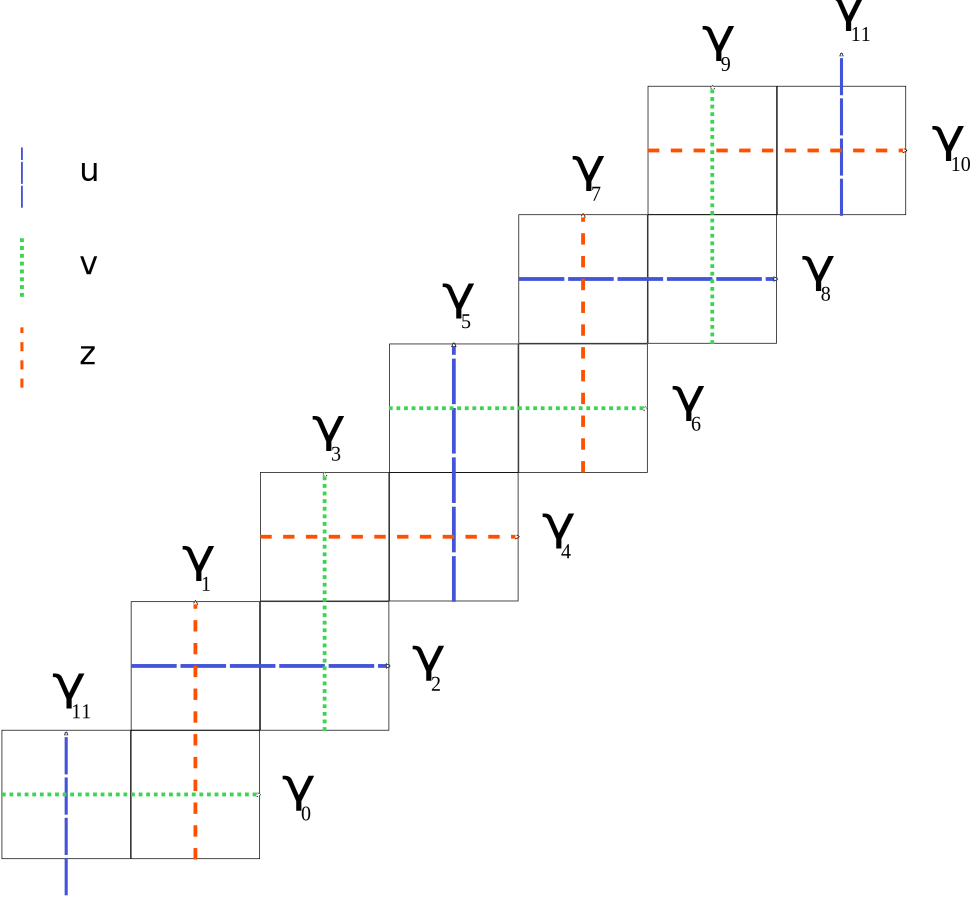
\includegraphics[width=3in]{homologyclass.png}
\centering
\caption{Cylinder core curves with u,v, and z homology classes that determines the $\mathbf{Z}^{2}$-cover.}
\label{fig:homology}
\end{figure}

\begin{Def}
The set of abelianized cylinder core curves is denoted as $\Gamma=\{\gamma_i: i = 0,\dots,11\}\subset H_1(\mathbf{M},\mathbb{Q})$.
\end{Def}

\begin{rem}
We use 12 elements to span homology, although a basis requires only 10. It's not impossible to determine the relations between these core curve classes, but it is not necessary. A $12\times12$ matrix of these core curve cylinder decompositions to their intersection numbers with adjacent curves is rank 10, as to be expected.
\end{rem}

The induced homomorphisms of $H_1(\mathbf{M}, \mathbb Q)$ have come from affine maps that have various effects on these core-curves. We use a 12-gon to represent the set of curves, and show how these elements act on them. The multi-twists add curves to adjacent curves, and the translation maps permute them. The reader is encouraged to check these for themselves.

e.g. for $\mathbf{H,V}\in$Aff$^+(\mathbf{M})$,

\begin{minipage}{0.5\textwidth}
\vspace{0.3in}
\begin{itemize}
\item[\textbf{\emph{$\mathbf{H}$ \& $\mathbf{V}$}}] The effect that these two translations have on the 12-gon is a reflection about these lines. Observed by keeping track of the squares and core curves after $\mathbf{H}$ and $\mathbf{V}$ have acted on $\mathbf{X}$.
\end{itemize}
\end{minipage}
\begin{minipage}{0.7\textwidth}
\begin{figure}[H]
\hspace{0.2in}\includegraphics[width=1.7in]{12gonHV.pdf}
\end{figure}
\end{minipage}

\begin{Def}
The induced homomorphisms of $H_1(\mathbf{M},\mathbb{Q})$ are obtained from the affine subgroup $\mathbb{X}$ and denoted $\mathbb{X}_*$. The associated homomorphisms on the spanning set $\Gamma$ are given as:
\begin{align*}
\mathbf{A}^k_*\circ[\gamma_i]=&[\gamma_i] + \frac{k}{2}(1-(-1)^i)([\gamma_{i-1}]+[\gamma_{i+1}])\\
\mathbf{B}^k_*\circ[\gamma_i]=&[\gamma_i] + \frac{k}{2}(1+(-1)^i)([\gamma_{i-1}]+[\gamma_{i+1}])\\
\mathbf{R}_*\circ[\gamma_i]=&(-1)^i[\gamma_{1-i\text{ mod }12}]\\
\mathbf{H}_*\circ[\gamma_i]=&[\gamma_{12-i\text{ mod }12}]\\
\mathbf{V}_*\circ[\gamma_i]=&[\gamma_{10-i\text{ mod }12}]
\end{align*}
\end{Def}

\begin{Def}
The homology classes $u,v,z$ are given as the following sums of core curves:
\begin{align*}
[u] &= -[\gamma_2] +[\gamma_5] + [\gamma_8] - [\gamma_{11}],\\
[v] &= +[\gamma_0] -[\gamma_3] -[\gamma_6] +[\gamma_9],\\
[z] &= +[\gamma_1] +[\gamma_4]-[\gamma_7]-[\gamma_{10}].
\end{align*}
\end{Def}

\begin{thm}
The fundamental group of the $\mathbb{Z}^2$-cover is obtained by lifting the kernel of the closed paths of $\mathbf{M}$ of the homomorphism:

\begin{align*}
\Omega_{u,v}:\pi_1(\mathbf{M},x_0)\rightarrow \mathbb{Z}^2 \text{; } \beta\mapsto(i(u,[\beta]),i(v,[\beta])),\text{ where}
\end{align*}

\begin{align*}
i:H_1(\mathbf{M},\mathbb Q)\times H_1(\mathbf{M},\mathbb Q)\rightarrow \mathbb Z.
\end{align*}is the intersection number of two homology classes.
\begin{proof}
We know from Theorem $\ref{thm:z2}$ that the translational symmetries of $\tilde{\mathbf{U}}$ induced by $T^{m,n}$ is isometric to $\mathbb{Z}^2$. Since $\mathbf{M}$ is a genus 5 base surface, we know that $\pi_1(\mathbf{M},x_0)\simeq \mathbb{Z}^{10}$, and the associated cover satisfies $\mathbf{M}=\tilde{\mathbf{U}}/(\pi_1(\mathbf{M},x_0)/N)$, such that $N$ is a normal subgroup of $\pi_1(\mathbf{M},x_0)$. This means that $N\simeq \mathbb{Z}^8$. The eight core curve classes are the abelianized forms of  $\gamma_0,\gamma_2,\gamma_3,\gamma_5,\gamma_6,\gamma_8,\gamma_9,$ and $\gamma_{11}$ that span N. The classes and their signs are obtained from Figure $\ref{fig:mtilda}$ as the outer regions identified by the translations of $T^{m,n}$. Thus any closed path on $\mathbf{M}$ is lifted to a closed path on the cover under the quotient map only when a path has a trivial intersection number with the classes.
\end{proof}

\end{thm}
Two paths are homologous if they return the same intersection number with the classes of closed core cylinder curves of $\mathbf{U}$ that span its homology. The classes u and v are obtained from the group group action of $T^{m,n}$ on the cover.

\begin{Def}
$\mathbf{hol}:\mathbf{M}\backslash\text{Sing}(\mathbf{M})\rightarrow\mathbb{C}$ is the holonomy vector pulled back from a non-singular path $\gamma$ in $\mathbf{M}$ onto the complex plane given by $\mathbf{hol}(\gamma)=\int_{\gamma}dz$.
\end{Def}

We denote the \textbf{closed path} $\alpha$, such that $\mathbf{hol}(\alpha)=6+6i$, and show it is homologous to the closed geodesic with the same holonomy vector. The slope one direction also decomposes $\mathbf{M}$ into two cylinders by a series of saddle connections of length $\sqrt{2}$ between singularities:

\begin{figure}[H]
\centering
\includesvg[width=4.4in.]{slopeonecylinder}
\caption{The two right-most cylinders $C_1$ (labeled) and $C_2$(unlabeled).}
\end{figure}

The circumferences of these two cylinders are $6\sqrt{2}$. Geodesic flows on this surface are well defined, and rational directions 

\begin{Def}
Let $\omega^{\theta}_t:[0,1]\times\mathbb{R}/2\pi\mathbb{Z}\rightarrow\mathbf{M}$ be the \textbf{maximal geodesic flow} on the surface in direction $\theta$ such that $\omega^{\theta}_0=\omega^{\theta}_1=x_0\in\mathbf{M}\backslash\text{Sing}(\mathbf{M})$.\\
$\omega^{\frac{\pi}{4}}_t$ is the geodesic flow in the \textbf{slope one direction}, and $\chi$ is its image in $\mathbf{M}$ and element of $\pi_1(\mathbf{M},x_0)$.
\end{Def}

\begin{lem}
$\alpha$ is homologous to $\chi$ in  $\mathbf{M}\backslash\text{Sing}(\mathbf{M})$.
\begin{proof}
Let $\chi$ be a geodesic contained in either $C_1$ or $C_2$. Since a geodesic does not admit singularities, it is the image of a closed path on $X\backslash\text{Sing}(X)$ with initial point $x_0$ on the strips of $C_1$ and $C_2$ with boundaries removed, denoted $C_1',$ $C_2'$. Express $[\alpha]$ as $\Sigma^{11}_{j=0}$ $\frac{1}{2}\gamma_j$ (a closed path climbing up the staircase). We show that the intersection numbers of $[\alpha]$ and $[\chi]$ are the same for every core cylinder curve $\gamma$, i.e. $i([\gamma_k], \Sigma^{11}_{j=0} \text{ } \frac{1}{2}[\gamma_j])=i([\gamma_k],[\chi])\text{ } \forall k=0,\dots,11$.\\
\textbf{Case one:} k is even. If k is even, then every curve $\gamma_k$ is oriented to the right. Since $\chi$ intersects every curve once, $i([\gamma_k],[\chi])=1$. No even indexed curves intersect eachother, so we need only consider when $j$ is odd. Now if $j$ is odd, it is incident (positively crossing) with only two horizontal curves, namely $\gamma_{j+1},\gamma_{j-1}$. Therefore $i([\gamma_k],[\alpha])=i([\gamma_{j-1}],\frac{1}{2}[\gamma_{j}])+i([\gamma_{j+1}],\frac{1}{2}[\gamma_{j}])=\frac{1}{2}(i([\gamma_{j-1}],[\gamma_{j}])+i([\gamma_{j+1}],[\gamma_{j}]))=\frac{1}{2}(1+1)=1.$\\
\textbf{Case two:} k is odd. If k is odd, then $[\chi]$ will have an intersection number of $-1$ with $[\gamma_k]$ since odd-indexed core curves are oriented upwards. Now since k is odd, we only consider when $j$ is even. Similarly, this means that $\gamma_j$ negatively intersects the two vertical core curves with adjacent indices. Hence, $i([\gamma_k],[\alpha])=i([\gamma_{j-1}],\frac{1}{2}[\gamma_{j}])+i([\gamma_{j+1}],\frac{1}{2}[\gamma_{j}])=\frac{1}{2}(i([\gamma_{j-1}],[\gamma_{j}])+i([\gamma_{j+1}],[\gamma_{j}]))=\frac{1}{2}(-1-1)=-1.$\\
We know intersection number to be bilinear and non-degenerate on homology. So if $\alpha$ and $\chi$'s abelianizations admit the same intersection numbers for every curve in the spanning set of $H_1(\mathbf{M}, \mathbb{Q})$, then $[\alpha]=[\chi]$.
\end{proof}
\end{lem}

\begin{thm}
$\chi\in\pi_1(\mathbf{M},x_0)$ lifts to $\tilde{\chi}\in\pi_1(\tilde{\mathbf{U}},\tilde{x}_0)$
\begin{proof}
From Lemma 2, $[\chi]=[\alpha]$, so $\Omega_{u,v}(\chi)=\Omega_{u,v}(\alpha)$. Since
$i([u],[\alpha])=-i([\gamma_2],[\alpha] +i([\gamma_5],[\alpha]) + i([\gamma_8],[\alpha]) - i([\gamma_{11}],[\alpha])=-1+(-1)+1-(-1)=0$ and $i([v],[\alpha])=1-(-1)-1+(-1)=0$, it follows that $\alpha,\chi\in\text{Ker }\Omega_{u,v}$, and $\chi$ lifts to a closed geodesic on $\tilde{\mathbf{U}}$.
\end{proof}
\end{thm}

\begin{cor}
content...
\end{cor}

From here, we use $\alpha$ to show that the \emph{only} trajectories that close on the Necker cube surface are those that are in vector direction $(a,b)$ such that $\gcd(a,b)=1$ and $a,b$ are both odd. We call these \textbf{odd-odd} directions. We can make this claim because the group generated by the matrices 

\begin{equation*}
\left[ \hspace{1mm} \begin{matrix}
				1 &  \pm 2\\
				0 & 1
			\end{matrix}\hspace{1mm}\right] \text{ and }
			\left[ \hspace{1mm} \begin{matrix}
							1 & 0\\
							 \pm 2 & 1
						\end{matrix}\hspace{1mm}\right]
\end{equation*}
is the \emph{Sanov subgroup} of $SL(2,\mathbb{Z})$ and only sends elements in the odd-odd set to itself. There are dualizations made between how these matrices skew a geodesic direction,  and how their original affine transformations induce an effect homology. In a sense the kernel is obtained by the orbit of $\chi$ under $\mathbb{X}$ and its holonomy vector under $\mathbb{X}'$.

\begin{lem}
The actions of $\mathbb{X}'$ on $\mathcal{O}$ and $\mathcal{E}$ are closed in their respective sets.
\begin{proof}
Since $\mathbb{X}'$ is generated by the elements $\mathbf{A}'$, $\mathbf{B}'$, and $\mathbf{R}'$, any matrix $G'\in\mathbb{X}'$ is of the form $G' = (\mathbf{A}')^{1_1}\circ(\mathbf{B}')^{1_2}\circ(\mathbf{R}')^{1_3}\circ(\mathbf{A}')^{2_1}\circ\dots(\mathbf{A}')^{n_1}\circ(\mathbf{B}')^{n_2}\circ(\mathbf{R}')^{n_3}$, where $i_k\in\mathbb{Z}$ for $i=1,\dots,n$ and $k=1,2,3.$ Let $x=\left(\begin{matrix}p \\ q  \end{matrix}\right),y\in\mathcal{O}$, and consider the equation $G'x=y$. Observe that $\left(\begin{matrix}1 && 2 \\ 0 && 1\end{matrix}\right)^l x=\left(\begin{matrix}p+2jq \\ q  \end{matrix}\right),$ and $ \left(\begin{matrix}1 && 0 \\ 2 && 1\end{matrix}\right)^m x=\left(\begin{matrix}p \\ q+2mp  \end{matrix}\right)$ for any $l,m\in\mathbb{Z}$. Also note that for any $j\in\mathbb{Z}$, $(\mathbf{R}')^{m}x=\left(\begin{matrix}p \\ q  \end{matrix}\right),\left(\begin{matrix}-q\\ p  \end{matrix}\right),\left(\begin{matrix}-p \\ -q  \end{matrix}\right),\left(\begin{matrix}q \\ -p  \end{matrix}\right)$ when $j \mod{4}\equiv0,1,2,3$, respectively. In any case, the product of any power of a generator of $\mathbb{X}'$ and any $x\in\mathcal{O}$ is an element of $\mathcal{O}$ . By letting $l=i_1,m=i_2,$ and $j=i_3$, we first consider the base case when $i=n$. Let $G'=G'_1\circ\dots\circ G'_n$, such that $G'_i=(\mathbf{A}')^{i_1}\circ(\mathbf{B}')^{i_2}\circ(\mathbf{R}')^{i_3}$. Since $n_1,n_2,n_3$ are arbitrary integers, $G'_n x \in\mathcal{O}$. Suppose for some $b< n-1$, $G'_{n-b}\circ\dots\circ G'_n x =y'\in\mathcal{O}$. Therefore $y'=(G'_1\circ\dots\circ G'_{b})^{-1}y$, which implies that $(G'_1\circ\dots\circ G'_{b})^{-1}$ preserves the set $\mathcal{O}$. Otherwise, if $y\in\mathcal{E}$, there exists at least one $G'_i$ for $1< i< b$ and $\tau\in\mathcal{E}$ such that $G'^{-1}_i \tau = (\mathbf{R}')^{-i_3}\circ(\mathbf{B}')^{-i_2}\circ(\mathbf{A}')^{-i_1} \tau \in \mathcal{O}$, a contradiction. Since elements in $\mathbb{X}'$ are invertible, $G'_1\circ\dots\circ G'_{b}$ must also map $\mathcal{O}$ to itself. Left multiply both sides of the equation to show that $G'_1\circ\dots\circ G'_n x = G' x = y$. By the principle of strong induction, this holds for all $0<b\leq n$. Since $G'$ is invertible and an arbitrarily chosen element of $\mathbb{X}'$, it follows that $x\in\mathcal{O}$ if and only if $y\in\mathcal{O}$ and $\mathcal{O}$ is closed under $\mathbb{X}'$.\\
The proof for when $x\in\mathcal{E}$ is made in the same way.
\end{proof}
\end{lem}


Now a trajectory in the horizontal direction has a directional vector of (1,0). The orbit of this vector by the Veech group is the set of all \textbf{even-odd} vectors. We also know that in this direction a geodesic is drift-periodic (See figure 1). The Veech group of $\mathbf{M}$ preserves these properties. Suppose you had some closed geodesic on $\mathbf{M}\backslash Sing(\mathbf{M})$ called $\beta$ such that $\beta=h(\alpha)$, where $h\in$  Aff$^+(\mathbf{M})$, and $h_*$ is its induced homomorphism. Then we want to show that

\begin{align*}
(i([\beta],[u]), i([\beta],[v]))=(i([\alpha],h^{-1}_*[u]), i([\alpha],h^{-1}_*[v])) = (0,0).
\end{align*}

But first, we look at some of the properties of the group $\mathbb{X}_*$.

\begin{thm}
Let $\mathbb{X}_*$ be the group generated by $\mathbf{A}_*, \mathbf{B}_*, \mathbf{R}_*, \mathbf{H}_*,$ and $\mathbf{V}_*$. Let $G=\left< \mathbf{A}_*, \mathbf{B}_* \right>$, $T=\left< \mathbf{H}_*, \mathbf{V}_* \right>$, and $R=\left< \mathbf{R}_*\right>$. Then the following is true:
\begin{enumerate}[label=(\roman*)]
\item $G$ is a free subgroup of $\mathbb{X}_*$ of rank two.
\item $T$ is a finite cyclic subgroup of $\mathbb{X}_*$ and a centralizer of G.
\item $R$ is a finite cyclic subgroup of $\mathbb{X}_*$, and a normalizer of $G$.
\end{enumerate}
\begin{proof} Let $h_*^{j}=\mathbf{A}_*^{k_j}\circ \mathbf{B}_*^{g_j}\in G$ for $k_j, g_j \in\mathbb{Z}$, $j=1,\dots,n$.\\ \emph{(i)}. When $\mathbf{A}_*$ and $\mathbf{B}_*$ act on $\gamma_i$, it is only ever trivial if i is even for $\mathbf{A}_*$ or i is odd on $\mathbf{B}_*$. Since i cannot be both odd and even at the same time, there is no relation between the two generators and therefore $G$ is free.\\
\emph{(ii)} It is up to the reader to show that $T$ has the relations $\mathbf{H}_*^2=\mathbf{V}_*^2=(\mathbf{H}_*\mathbf{V}_*)^3=id_*$, and is isomorphic to the rotational group of the hexagon generated by reflections about adjacent vertices of a 12-gon. Observe that $\mathbf{H}_*\circ \mathbf{A}_*^{k_j}\circ[\gamma_i]=\mathbf{H}_*\circ[\gamma_i] + \frac{k_j}{2}(1-(-1)^i)(\mathbf{H}_*\circ[\gamma_{i-1}]+\mathbf{H}_*\circ[\gamma_{i+1}])=[\gamma_{-i}] + \frac{k_j}{2}(1-(-1)^i)([\gamma_{1-i}]+[\gamma_{-i-1}])=\mathbf{A}^{k_j}\circ[\gamma_-i]=\mathbf{A}^{k_j}\circ\mathbf{H}_*\circ[\gamma_i],$ and $\mathbf{V}_*\circ \mathbf{A}_*^{k_j}\circ[\gamma_i]=\mathbf{V}_*\circ[\gamma_i] + \frac{k_j}{2}(1-(-1)^i)(\mathbf{V}_*\circ[\gamma_{i-1}]+\mathbf{V}_*\circ[\gamma_{i+1}])=[\gamma_{10-i}] + \frac{k_j}{2}(1-(-1)^i)([\gamma_{11-i}]+[\gamma_{9-i}])=\mathbf{A}^{k_j}\circ[\gamma_10-i]=\mathbf{A}^{k_j}\circ\mathbf{V}_*\circ[\gamma_i].$ In the same way one can show this to be true for $\mathbf{B}_*^{g_j}$, and we can see that $T$ is a centralizer of $G$. \\
\emph{(iii)} $R$ is obviously cyclic and finite since an isomorphism is obtained as $\mathbf{R}_*\mapsto\mathbf{R}'\in SO(2,\mathbb{Z})$. \\Note that $\mathbf{R}_*\circ\mathbf{A}_*^{k_j}\circ[\gamma_i]=\mathbf{R}_*\circ[\gamma_i] + \frac{k_j}{2}(1-(-1)^i)(\mathbf{R}_*\circ[\gamma_{i-1}]+\mathbf{R}_*\circ[\gamma_{i+1}])\\
=(-1)^i[\gamma_{1-i}] + \frac{k_j}{2}(1-(-1)^i)((-1)^{i-1}[\gamma_{2-i}]+(-1)^{i+1}[\gamma_{-i}])\\
=(-1)^{1-i}([\gamma_{1-i}] - \frac{k_j}{2}(1+(-1)^{1-i})([\gamma_{2-i}]+[\gamma_{-i}]))\\
=(-1)^{1-i}\mathbf{B}_*^{-k_j}\circ[\gamma_{1-i}]=\mathbf{B}_*^{-k_j}\circ(-1)^{1-i}[\gamma_{1-i}]=\mathbf{B}_*^{-k_j}\circ\mathbf{R}_*\circ[\gamma_{i}].$\\
Likewise, $\mathbf{R}_*\circ\mathbf{B}_*^{g_j}\circ[\gamma_{i}]=\mathbf{A}_*^{-g_j}\circ\mathbf{R}_*\circ[\gamma_{i}]$.
\end{proof}
\end{thm}

\begin{rem}
It can be easily shown that $\mathbb{X}'$ has similar properties.
\end{rem}


\begin{lem}
$Let$ $h_*\in \left<\mathbf{A}_*,\mathbf{B}_*\right>. $ Then $h_*\circ[\alpha]\in H_1(\mathbf{M},\mathbb{Q})$ can be expressed as $h_*\circ[\alpha]=\frac{1}{2}(c_1\Sigma^{5}_{j=0}[\gamma_{2j}]+c_2\Sigma^{5}_{j=0}[\gamma_{2j+1}])$ for $c_1,c_2\in\mathbb{Z}$.
\begin{proof}
Let $\Sigma^{5}_{j=0}[\gamma_{2j}]=\Sigma\Gamma_{even}$, $\Sigma^{5}_{j=0}[\gamma_{2j+1}]= \Sigma\Gamma_{odd}$, and  $\Sigma^{11}_{j=0}[\gamma_{j}]= \Sigma\Gamma$. Let $h_*=h_*^n\circ\dots\circ h_ *^1$, and $h_*^{i}=\mathbf{A}_*^{k_i}\circ \mathbf{B}_*^{g_i}$ for $k_i, g_i \in\mathbb{Z}$, $i=1,\dots,n$. Compose these two homomorphisms and obtain $\mathbf{A}_*^{k_i}\circ \mathbf{B}_*^{g_i}(\Sigma\Gamma)=(4g_ik_i+2k_i)\Sigma\Gamma_{even}+2g_i\Sigma\Gamma_{odd}+\Sigma\Gamma$. Let $c_i^1=(4g_ik_i+2k_i), c_i^2=2g_i$, and solve for $h_*^{i+1}\circ h_*^i\circ\Sigma\Gamma$:
\begin{align*}
h_*^{i+1}\circ h_*^{i}\circ(\Sigma\Gamma)=h_*^{i+1}\circ(c_i^1\Sigma\Gamma_{even}+c_i^2\Sigma\Gamma_{odd}+\Sigma\Gamma)\\ =c_i^{1}h_*^{i+1}\circ(\Sigma\Gamma_{even})+c_i^2h_*^{i+1}\circ(\Sigma\Gamma_{odd})+h_*^{i+1}\circ(\Sigma\Gamma)\\ =2g_{i+1}\Sigma\Gamma_{odd}+(4g_{i+1}k_{i+1}+2k_{i+1})\Sigma\Gamma_{even}+\Sigma\Gamma\\+c_i^{1}(4g_{i+1}k_{i+1}\Sigma\Gamma_{even}+2g_{i+1}\Sigma\Gamma_{odd}+\Sigma\Gamma_{even})\\+c_{i}^2(2k_{i+1}\Sigma\Gamma_{even}+\Sigma\Gamma_{odd})\\
=\Sigma\Gamma+(c_i^1+(c_{i}^1+1)(4g_{i+1}k_{i+1})+(c_i^2+1)2k_{i+1})\Sigma\Gamma_{even}\\+(c_i^2+(c_i^1+1)2g_{i+1})\Sigma\Gamma_{odd}\\
\text{Let }c_{i+1}^1:=(c_i^1+(c_{i}^1+1)(4g_{i+1}k_{i+1})+(c_i^2+1)2k_{i+1}),\\
c_{i+1}^2:=(c_i^2+(c_i^1+1)2g_{i+1}).
\end{align*}
From these recursive definitions and a finite sequence of integers, $\{k\}_i,\{g\}_i$, observe then that\\ $h_*\circ[\alpha]=h_*\circ[\frac{1}{2}\Sigma\Gamma]=\frac{1}{2}h_*\circ[\Sigma\Gamma]=\frac{1}{2}[c_n^1\Sigma\Gamma_{even}+c_n^2\Sigma\Gamma_{odd}+\Sigma\Gamma]\\
=\frac{1}{2}[(c_n^1+1)\Sigma\Gamma_{even}+(c_n^2+1)\Sigma\Gamma_{odd}]$. Further simplify by letting $c_1=c_n^1+1,c_2=c_n^2+1$.
\end{proof}
\end{lem}

\begin{lem}
Let $h_*\circ[\alpha]\in H_1(\mathbf{M},\mathbb{Q})$. Then for $a\in\left<\mathbf{H}_*, \mathbf{V}_*\right>$ and $b\in\left<\mathbf{R}_*\right>$, the following is true:
\begin{align*}
& a\circ h_*\circ[\alpha]=h_*\circ[\alpha]\\
& b\circ h_*\circ[\alpha]=\frac{1}{2}[c'_1\Sigma\Gamma_{even}+c'_2\Sigma\Gamma_{odd}]\\
& h_*\circ b\circ[\alpha]=\frac{1}{2}[c''_1\Sigma\Gamma_{even}+c''_2\Sigma\Gamma_{odd}]
\end{align*}
\begin{proof}
By Theorem 4, a is a centralizer of the group so $a\circ h_*\circ[\alpha]=h_*\circ a \circ[\alpha]=h_*\circ \frac{1}{2}a \circ[\Sigma\Gamma].$ Since a is a cyclic permutation of the set $\Gamma$, it acts trivially on $\Sigma\Gamma$. Therefore, $a\circ h_*\circ[\alpha]=h_*\circ \frac{1}{2}[\Sigma\Gamma]=h_* \circ[\alpha]$.\\
By theorem 4, $a\circ\mathbf{A}_*^{k_i}\circ\mathbf{B}_*^{g_i}=\mathbf{B}_*^{-k_i}\circ\mathbf{A}_*^{-g_i}\circ a$. Extend this property to $h_*$, and denote the normalized element as $h_{**}$, such that $b\circ h_{*}=h_{**}\circ b$.  Note that $b(\Sigma\Gamma)=b(\Sigma\Gamma_{even}+\Sigma\Gamma_{odd})=\Sigma\Gamma_{odd}-\Sigma\Gamma_{even}$. $b\circ h_*\circ[\Sigma\Gamma]=c_1b\circ\Sigma\Gamma_{even}+c_2b\circ\Sigma\Gamma_{odd}=c_1\Sigma\Gamma_{odd}-c_2\Sigma\Gamma_{even}.$ So, $c_1'=-c_2$ and $c_2'=c_1$.\\
Since $h_*$ is arbitrary, let $h_{**}=g_{*}$ be generated by an integer sequence that defines the word and consider $h_*\circ b\circ[\Sigma\Gamma]=b\circ g_{*}\circ[\Sigma\Gamma]=c^*_1b\circ\Sigma\Gamma_{even}+c^*_2b\circ\Sigma\Gamma_{odd}=c^*_1\Sigma\Gamma_{odd}-c_2^*\Sigma\Gamma_{even}.$ So, $c_1''=-c_2^*$ and $c_2''=c_1^*$.
\end{proof}
\end{lem}

\noindent Now that every element in the orbit of $[\alpha]$ can be expressed as a linear combination of integers, it is simple to show they lift to a closed trajectory in the cover.

\begin{Def}
Let $\mathbf{dir}:UT(\mathbf{M}\backslash\text{Sing}(\mathbf{M}))\rightarrow\mathcal{O}\cup\mathcal{E}$ be the injective map from $\mathbb{R}/2\pi\mathbb{Z}$ to $\mathbb{Z}^2$ given as $\mathbf{dir}(\theta)=(k_1\cos(\theta),k_2\sin(\theta)), k_1,k_2\in\mathbb{R}$ such that $\gcd(k_1\cos(\theta),k_2\sin(\theta))=1$.
\end{Def}

\begin{thm}(Sketch)\\
Any geodesic, $\beta$, in $\mathbf{M}$ lifts to a closed geodesic $\tilde{\beta}$ on $\tilde{\mathbf{U}}$ if and only if $\mathbf{dir}(Arg(\mathbf{hol}(\beta)))\in\mathcal{O}$.
\begin{proof}
Call the quotient cover $p:\tilde{\mathbf{U}}\rightarrow\mathbf{M}$, and fix a point $\tilde{x_0}\in p^{-1}(x_0)$. Let $\beta=h(\chi)$, where $h\in\mathbb{X}$. We also obtain $[\beta]=h_*\circ[\alpha]$ from Lemma 2. Since $h$ sends geodesics to geodesics, h induces the following: $\mathbf{hol}(h(\chi))=h'(\mathbf{hol}(\chi))=h'(6+6i)$ for $h'=\left[\begin{matrix} a & b \\ c & d\end{matrix}\right]\in\mathbb{X}'$. So, Arg$(h'(\mathbf{hol}(\chi)))=$Arg$(6[(a+b)+i(c+d)])=$Arg$(6h'(1+i))$. Lemma 3 states that for any $h'\in\mathbb{X}'$, $h'(\mathcal{O})=\mathcal{O}$. Therefore there is no such geodesic of \textbf{even-odd} slope in the orbit of $\chi$. Otherwise $h',h\notin\mathbb{X}',\mathbb{X}$. Consequently, $\mathbf{dir}(Arg(\mathbf{hol}(\beta)))\in\mathcal{O}$.\\
From Lemma 5 we see that $[h(\chi)]=h_*\circ[\chi]=h_*\circ[\alpha]=\frac{1}{2}(c_1\Sigma^{5}_{j=0}[\gamma_{2j}]+c_2\Sigma^{5}_{j=0}[\gamma_{2j+1}])$ for $c_1,c_2\in\mathbb{Z}$. Denote the sums as $\Sigma\Gamma_{even}$ and $\Sigma\Gamma_{odd}.$\\
Therefore, $2i([u],h_*\circ[\alpha])=c_1i([u],\Sigma\Gamma_{even})+c_2i([u],\Sigma\Gamma_{odd})\\
=c_1(-i([\gamma_2],0) +i([\gamma_5],[\gamma_6]+[\gamma_4]) + i([\gamma_8],0) - i([\gamma_{11}],[\gamma_{10}]+[\gamma_{0}]))\\
+c_2(-i([\gamma_2],[\gamma_1]+[\gamma_3]) +i([\gamma_5],0) + i([\gamma_8],[\gamma_7]+[\gamma_9]) - i([\gamma_{11}],0))\\
=c_1(-(0)+(-1-1)+(0)-(-1-1))+c_2(-(1+1)+(0)+(1+1)-(0))=0.$\\\vspace{0.1in}\\
Similarly, $2i([v],h_*\circ[\alpha])=c_1i([v],\Sigma\Gamma_{even})+c_2i([v],\Sigma\Gamma_{odd})\\
=c_1(i([\gamma_0],0)-i([\gamma_3],[\gamma_2]+[\gamma_4])-i([\gamma_6],0)+i([\gamma_9],[\gamma_8]+[\gamma_{10}])\\
+c_2(i([\gamma_0],[\gamma_{11}]+[\gamma_1])-i([\gamma_3],0)-i([\gamma_6],[\gamma_5]+[\gamma_7])+i([\gamma_9],0)\\
=c_1((0)-(-2)-(0)+(-2))+c_2((2)-(0)-(2)+(0))=0.$\\
Therefore, $\Omega_{u,v}(h(\chi))=(0,0)$, and $h(\chi)=\beta\in\text{Ker }\Omega_{u,v}$ for all $h\in\mathbb{X}$. By Theorem 2, $\beta$ lifts to $\tilde{\beta}\in\pi_1(\tilde{\mathbf{U}},\tilde{x}_0)$. Let $\theta=$Arg$(\mathbf{hol}(\beta))$. Then $\omega_t^{\theta}$ at $x_0$ lifts to $\tilde{\omega}_t^{p^{-1}(\theta)}\in\tilde{\mathbf{U}}\backslash\text{Sing}(\tilde{\mathbf{U}})$.\\
Now suppose instead that $\beta=h(\gamma_{i})$. Then $\mathbf{dir}(\beta)=\frac{1}{2}(1+(-1)^i,1-(-1)^i)$. According to Lemma 3, $h'(\mathcal{E})=\mathcal{E}$. Thus we have no geodesic in the \textbf{odd-odd} directions obtained from the orbits of $(1,0)$ and $(0,1)$. For contradiction, suppose that $h(\gamma_{i})\in\textbf{Ker }\Omega{u,v}$. Then $(i(h_*\circ[\gamma_i], [u]),i(h_*\circ[\gamma_i], [v]))=(i([\gamma_i], h^{-1}_*\circ[u]),i([\gamma_i], h^{-1}_*\circ[v]))=(0,0).$ Let $h^{-1}_*\circ[u]=\Sigma^{11}_{j=0}x_j[\gamma_j]$, and $h^{-1}_*\circ[v]=\Sigma^{11}_{j=0}y_j[\gamma_j]$. Note that since $\gamma_i$ intersects $\gamma_{i\pm1}$, $i([\gamma_i], h^{-1}_*\circ[u])=(-1)^{i+1}(x_{i-1}+x_{i+1})$ and $i([\gamma_i], h^{-1}_*\circ[v])=(-1)^{i+1}(y_{i-1}+y_{i+1}).$
\\
$\mathbf{Unfinished.}.$
\end{proof}
\end{thm}

\begin{conj}{\textbf{Dynamics of Geodesic Flow on the Necker cube surface.}}\\ Obtain $\theta$ and $\vec{\theta}$ as described in Definition 3. Denote the non-singular unit-speed geodesic flow with initial point $s\in(\mathbf{U}\backslash Sing(U))$ in direction $[\theta]\sim\phi\in UT(\mathbf{U}\backslash Sing(\mathbf U))$ by $F_t^{\phi}:\mathbf{U}\times\mathbb{R}_0^+\rightarrow\mathbf{U}$ on $(\mathbf{U},\mu)$, where $\mu$ is a flow-invariant measure.  Then the following is true:
\begin{enumerate}[label=(\roman*)]
\item (Periodic) There exists a $t_0 > 0$ such that $F^{\phi}_{t+t_{0}}(s)=F^{\phi}_{t}(s)$ if and only if $\vec{\theta}\in\mathcal{O}$.
\item (Drift-Periodic) There exists a $t_0 > 0$ such that $F^{\phi}_{t+t_{0}}(s)= F^{\phi}_{t}(s)+c$, where $c\in \mathbf{U}$ is a non-trivial translation of a point in $\mathbf{U}$, if and only if $\vec{\theta}\in\mathcal{E}$.
\end{enumerate}
\begin{proof}(Sketch)\\
Denote the covering maps $f:\tilde{\mathbf{U}}\rightarrow\mathbf{U}$, $p:\tilde{\mathbf{U}}\rightarrow\mathbf{M}$, and fix a point $\tilde{x}_0\in f^{-1}(s),p^{-1}(x_0),$ for $x_0\in\mathbf{M}$. $f^{-1}([\theta])=\{x:x=\theta+n\frac{\pi}{2}, n\in\mathbb{Z}\}=[\theta]\subset UT(\tilde{\mathbf{U}}\backslash\text{Sing}(\tilde{\mathbf{U}}))$ given by the four-fold cover and rotations of each individual plane. This gives us a relation between the two tangent bundles, where the translation four-fold cover has the standard $\mathbb{R}/2\pi\mathbb{Z}$ unit tangent fiber. $\theta'$ is the direction associated to the flow $\omega_t^{\theta'}:[0,1]\rightarrow\mathbf{M}$ on the translation surface. Since the cover is translation, $p^{-1}(\theta')=\theta'=\theta+n\frac{\pi}{2}$.  First suppose that $\vec{\theta}\in\mathcal{O}$. Then $\theta$ is identified with the set of directions that close on $\tilde{\mathbf{U}}$. From Theorem 5, $\omega_t^{\theta'}$ lifts to a closed geodesic $\tilde{\omega}_t^{\theta'}$. Given $\mathbf{hol}(\omega)=\int_{\omega}dz$, we obtain a period for the unit-speed flow, $t_0=|\mathbf{hol}(\omega)|$. That is, $\tilde{F}_t^{\theta'}:\mathbb{R}^+_0\rightarrow\tilde{\mathbf{U}}$ such that  $\frac{d}{dt}\tilde{F}_t=\frac{1}{|\mathbf{hol}(\omega)|}$. Then $F_t^{\phi}=F_t^{[\theta']}=f\circ \tilde{F}^{\theta'}_t$. The period carries over since there is no concern over a trajectory returning to $\tilde{x_0}$ in a different direction. Otherwise, the geodesic $\omega_t^{\theta'}$ on $\mathbf{M}$ would have closed in $0<t<1$. Now suppose that $\vec{\theta}\in\mathcal{E}$. Identifying it with $\theta'$, we see that $\omega$ in direction $\theta'$ is not an element of $\textbf{Ker }\Omega_{u,v}$ from Theorem 5. Therefore, $\Omega_{u,v}(\omega)=(m,n)\simeq T^{m,n}$ and lifting the terminal point $\omega(1)$, $\tilde{\omega}(1)=T^{m,n}(\tilde{\omega}(0))=T^{m,n}(\tilde{x}_0).$ The period remains unchanged, in that $\tilde{F}^{\theta'}_{t+\mathbf{hol}(\omega)}=\tilde{F}^{\theta'}_{t}+T^{m,n}(\tilde{x}_0)$. Therefore, $F^{\phi}_{t+t_{0}}(s)=f\circ\tilde{F}^{\theta'}_{t}(\tilde{x}_0)+f\circ T^{m,n}(\tilde{x}_0).$\\
Conversely, suppose $F_t$ is periodic. Then $[\theta]=\phi=[\theta']$, which defines directional flows $\tilde{F}^{\phi}_t$. According to Theorem 5, $\tilde{F}^{\phi}_t$ will close if and only if $\phi\subset\mathcal{O}$. $\phi$ is the orbit of $\vec{\theta}'$ under the 90 degree rotational matrix. This matrix does not alter the length or period of a geodesic. Thus, $F^{\phi}_t$ is exactly one of the flows $\tilde{F}^{\phi}_t$. Likewise, if $F^\phi_t$ is drift-periodic then $F^\phi_{t+t_0}=f\circ \tilde{F}^\phi_t+f\circ T^{m,n}$. $T^{m,n}$ is trivial if and only if $\theta'\in\mathcal{O}$. Therefore, $\theta'\in\mathcal{E}$, and $[\theta']=\phi$.
\end{proof}
\end{conj}

There is still much work to do in terms of cleaning up the proofs and organizing the final paper.

\newpage
\section*{Conclusion}
What I ultimately aim to do is port these results on X's homology back to the Necker cube surface. I want do it in such a way that the final theorem is bi-conditional. To do so, I imagine I can take a vector image of a small segment of a geodesic in $\mathbb{R}^3$ and project it onto the isometric flattening of the Necker Cube surface to obtain a direction (or classes of equivalent directions), and relate it to the unit tangent bundle of $\mathbf{M}$.

In addition, I would also like to find a formula for the arc-length of a geodesic based on direction alone. Knowing that hol$(\alpha)=6+6i$ means that the induced Euclidean metric on $\mathbf{M}\backslash$Sing($\mathbf{M}$) gives the geodesic an arc-length of $6\sqrt{2}$. I would like to show that:

\begin{align*}
\int_{\beta}|dz|=|hol(h(\alpha))|=|h'(hol(\alpha))|,
\end{align*}
\noindent where $h'\in V(\mathbf{M})$ is the derivative of h, and $\beta=h(\alpha)$. We know that is true on the translation surface, but it's a matter of then showing the translation quotient, branch-cover, and the Necker cube surface have the same induced Euclidean metric of these non-singular geodesics. (It would not be surprising considering that the surface is built out of subsets of planes.) Even more of a problem is finding a way to solve for a matrix in the Sanov subgroup that brings (1,1) to the desired odd-odd slope.

Even though the main theorem remains unproven for now, it is an enjoyable property of the surface and venturing in its understanding involves exploring some fascinating niches in algebraic topology and dynamical systems.

Needless to say, it has been a very busy summer for me. I am grateful for the opportunity to really take some time to delve deep into numerous topics that I have been very interested in for a while. I sincerely doubt it would have been possible without the summer internship, and I have the Rich scholarship committee to thank for that. I would also like to extend my gratitude to Dr. Hooper. He has been incredibly patient and kind throughout these last few months, and I would not have come this far in so short a time without his help. 


\newpage
\begin{thebibliography}{9}
\bibitem{Robotics} Fred G. Martin \emph{Robotics Explorations: A Hands-On Introduction to Engineering}. New Jersey: Prentice Hall.
\bibitem{Flueck}  Flueck, Alexander J. 2005. \emph{ECE 100}[online]. Chicago: Illinois Institute of Technology, Electrical and Computer Engineering Department, 2005 [cited 30
August 2005]. Available from World Wide Web: (http://www.ece.iit.edu/~flueck/ece100).
\end{thebibliography}
\end{document}          
